\pagebreak

\subsection{Strumenti adottati}
\label{sez:strumenti-adottati}

\subsubsection{Strumenti organizzativi}
\label{sez:strumenti-organizzativi}

\noindent \textbf{Jira\\}

\noindent \textit{Jira} è un \gls{its} che permette la gestione delle attività di progetto in modo \textit{Agile}, fa parte della suite di prodotti di \textit{Atlassian}.\\
Un \gls{its} permette ai membri del team di visualizzare le attività assegnate, aggiornare lo stato di avanzamento e comunicare con gli altri membri del \textit{team} sul lavoro svolto. \\
Durante lo \textit{stage} l'ho utilizzato per la creazione di \textit{epic} e \textit{stories}, delle loro sotto \textit{task}, la pianificazione delle attività ed il tracciamento dei requisiti. \\
Nella {\hyperref[fig:jira-list-stories]{Figura 1.1}} si possono vedere alcune delle \textit{stories} che ho creato durante la fase di pianificazione.
\begin{figure}[H]
    \label{fig:jira-list-stories}
    \centering
    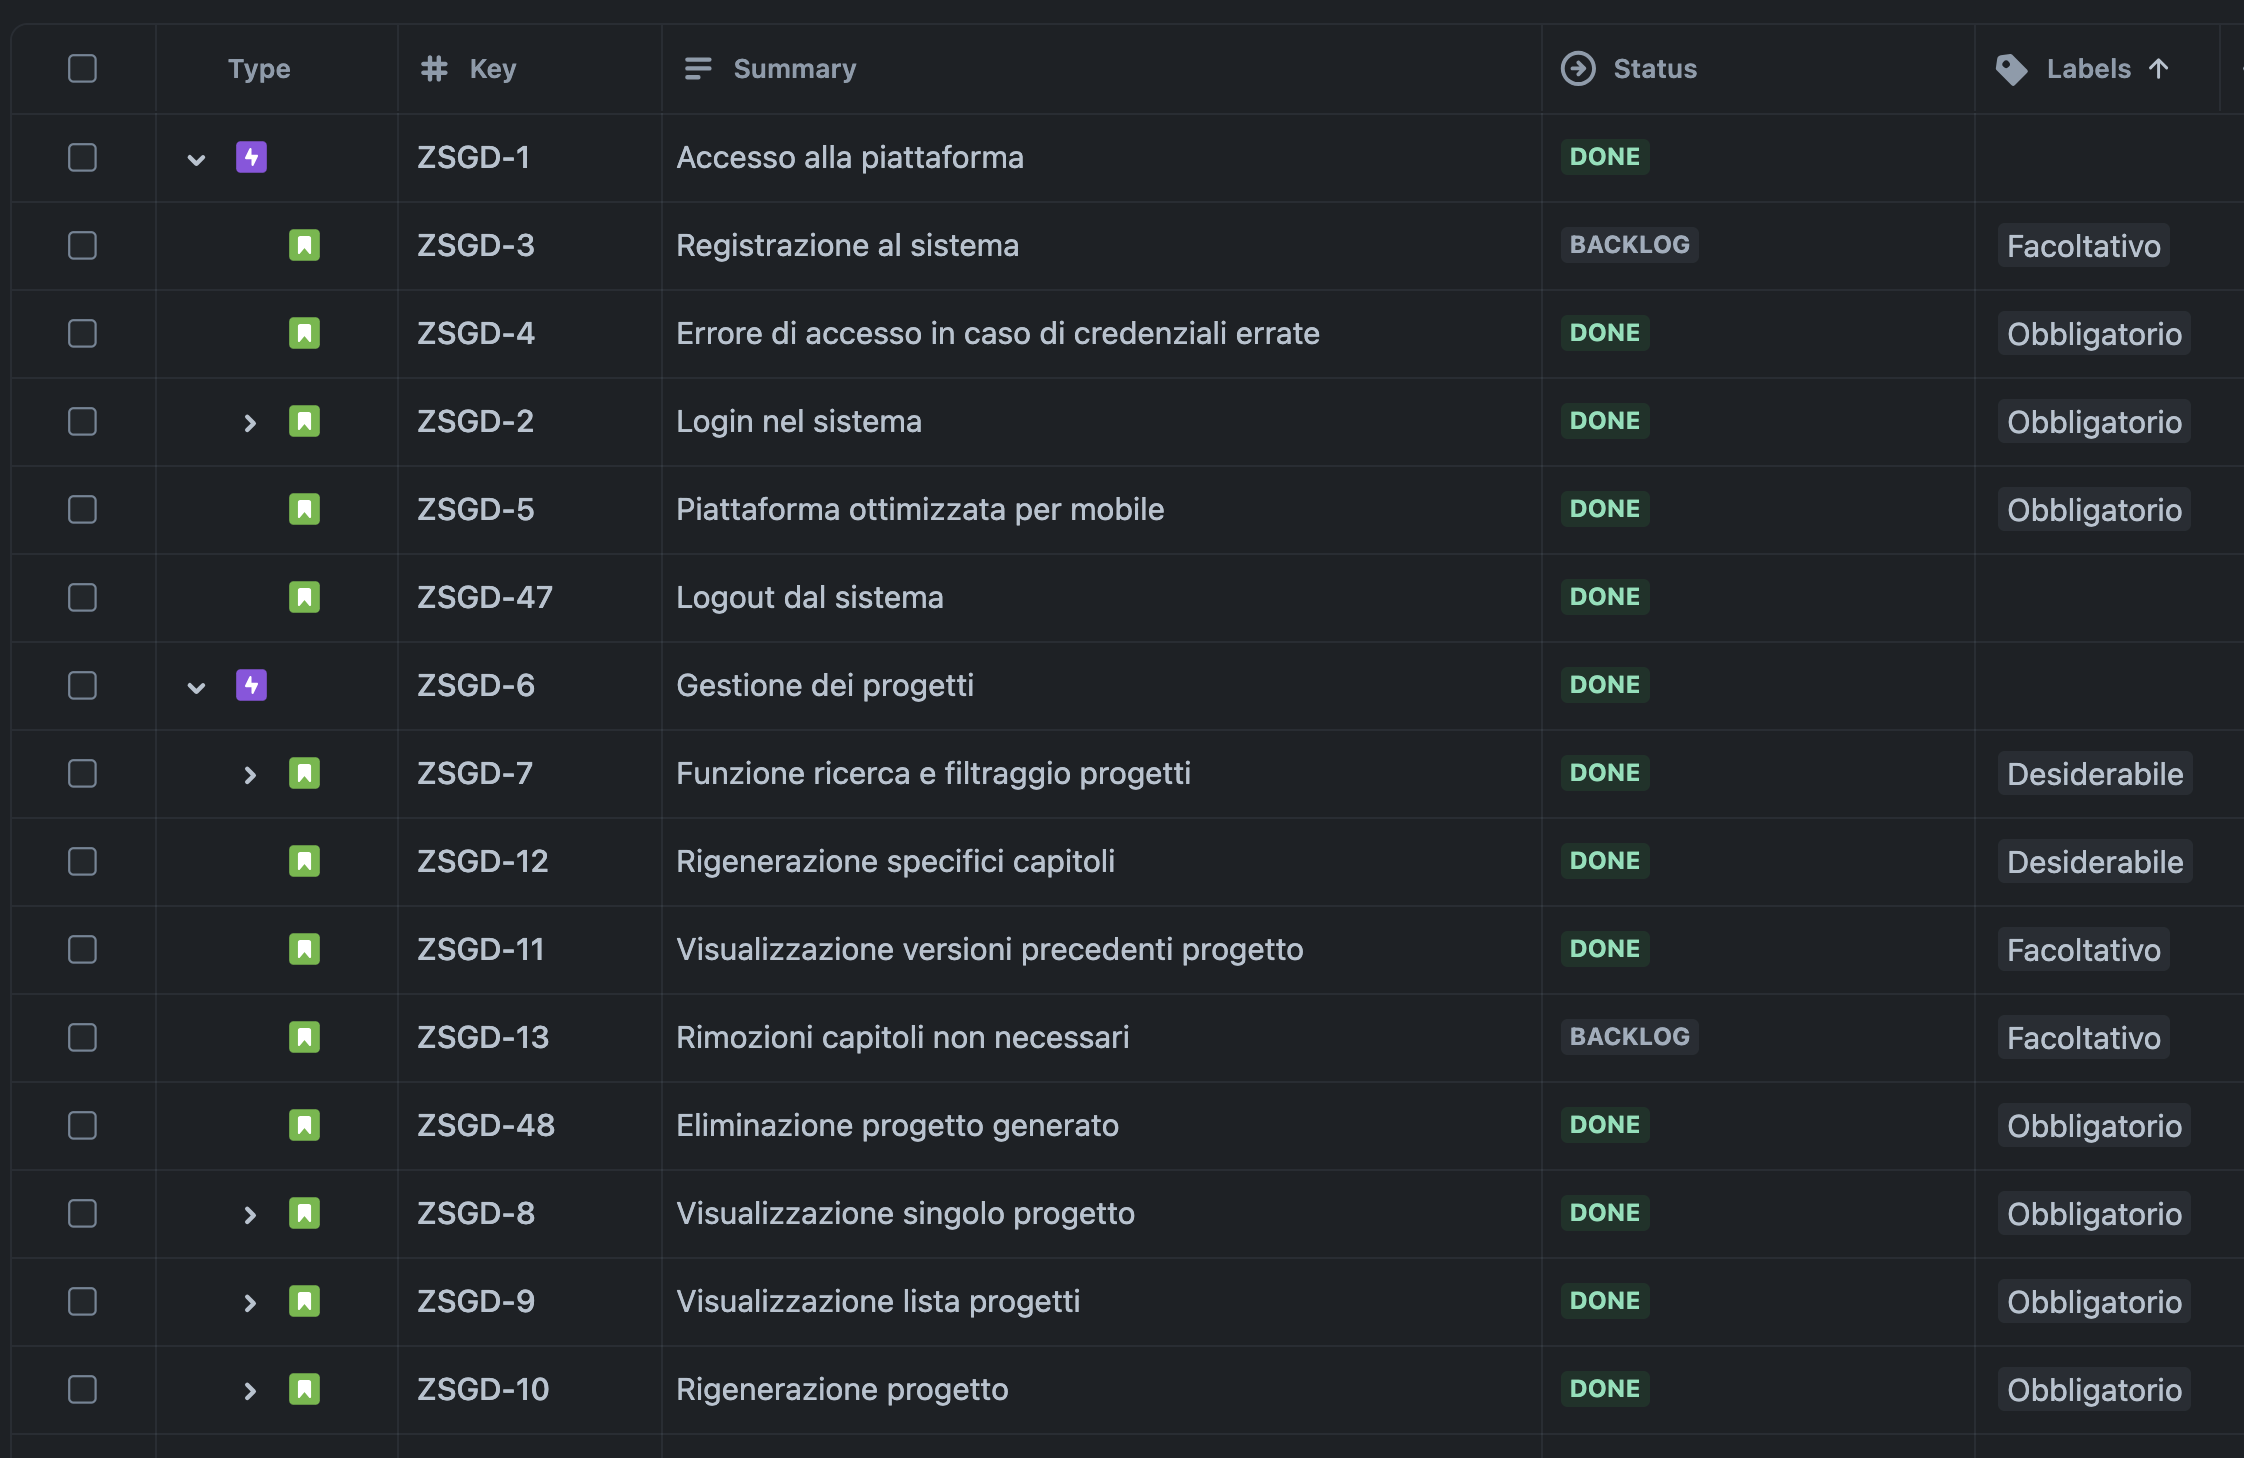
\includegraphics[scale=0.3]{strumenti/jira-list-stories.png}
    \caption{\textit{Jira} - Lista delle \textit{stories}}
\end{figure}

\noindent \textbf{Confluence\\}

\noindent \textit{Confluence} è un'applicazione di collaborazione che permette la creazione di documentazione in modo collaborativo tra i componenti di un \textit{team} di lavoro, fa parte della suite di prodotti di \textit{Atlassian}.\\
Durante lo \textit{stage} l'ho utilizzato per la creazione di documentazione relativa al progetto, come ad esempio la documentazione tecnica ed il documento di analisi progettuale.\\

\pagebreak
\noindent \textbf{Visual Studio Code\\}

\noindent \textit{Visual Studio Code} (da qui in poi \textit{VSCode}) è un \gls{ide} sviluppato da \textit{Microsoft}, che permette la scrittura del codice in diversi linguaggi di programmazione, è stato utilizzato per andare
a sviluppare tutto il codice del progetto utilizzando il linguaggio \textit{TypeScript}.\\
Un \gls{ide} permette di scrivere, testare ed effettuare il \textit{debugging} del codice in un'unica applicazione, fornendo strumenti per facilitare lo sviluppo del \textit{software}; \textit{VSCode} è uno degli \gls{ideg} più utilizzati.\\
Nella {\hyperref[fig:vscode]{Figura 1.2}} è possibile vedere l'interfaccia di sviluppo di \textit{VSCode}, il codice mostrato è relativo alla funzione di generazione di un progetto.

\begin{figure}[H]
    \label{fig:vscode}
    \centering
    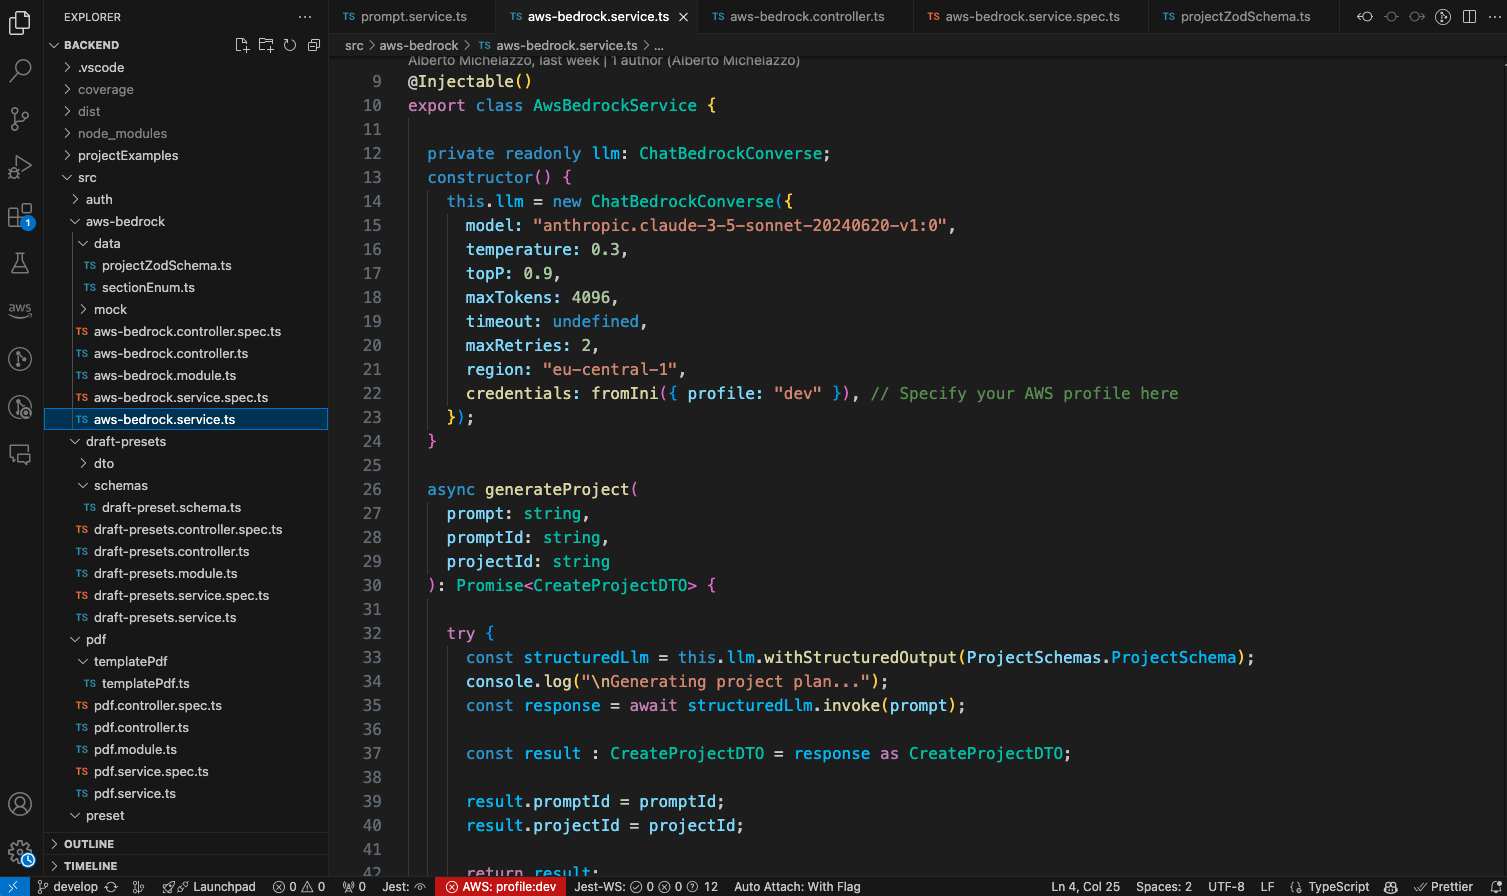
\includegraphics[scale=0.25]{strumenti/vscode.png}
    \caption{\textit{VSCode} - Interfaccia di sviluppo}
\end{figure}

\noindent \textbf{GitHub\\}

\noindent \textit{GitHub} è una piattaforma di \textit{hosting} per progetti \textit{software} che utilizzano il sistema di controllo di versione \textit{Git}.
Grazie a questa piattaforma è possibile andare a creare \textit{repositories} per il proprio progetto, permettendo la collaborazione tra i membri del \textit{team} ed il tracciamento delle modifiche effettuate. \\
È inoltre possibile andare a suddividere il progetto in \gls{branch}, per andare a sviluppare le funzionalità tramite cosidetti \textit{feature branch}.\\
Un \gls{branch} è una copia del codice principale del progetto, che permette di sviluppare nuove funzionalità senza influenzare il codice principale.\\
Terminata la codifica di una \textit{feature}, è possibile effettuare una \gls{pr} per andare ad unire il codice sviluppato con il \gls{branch} principale, dopo la revisione da parte di un collega.\\
Una \gls{pr} permette di discutere delle modifiche effettuate, garantire che il codice sia conforme alle \textit{best practices} del progetto e che non siano presenti errori.\\
Nella {\hyperref[fig:github]{Figura 1.3}} è possibile vedere una delle \textit{repositories} che ho creato per il progetto.

\begin{figure}[H]
    \label{fig:github} 
    \centering
    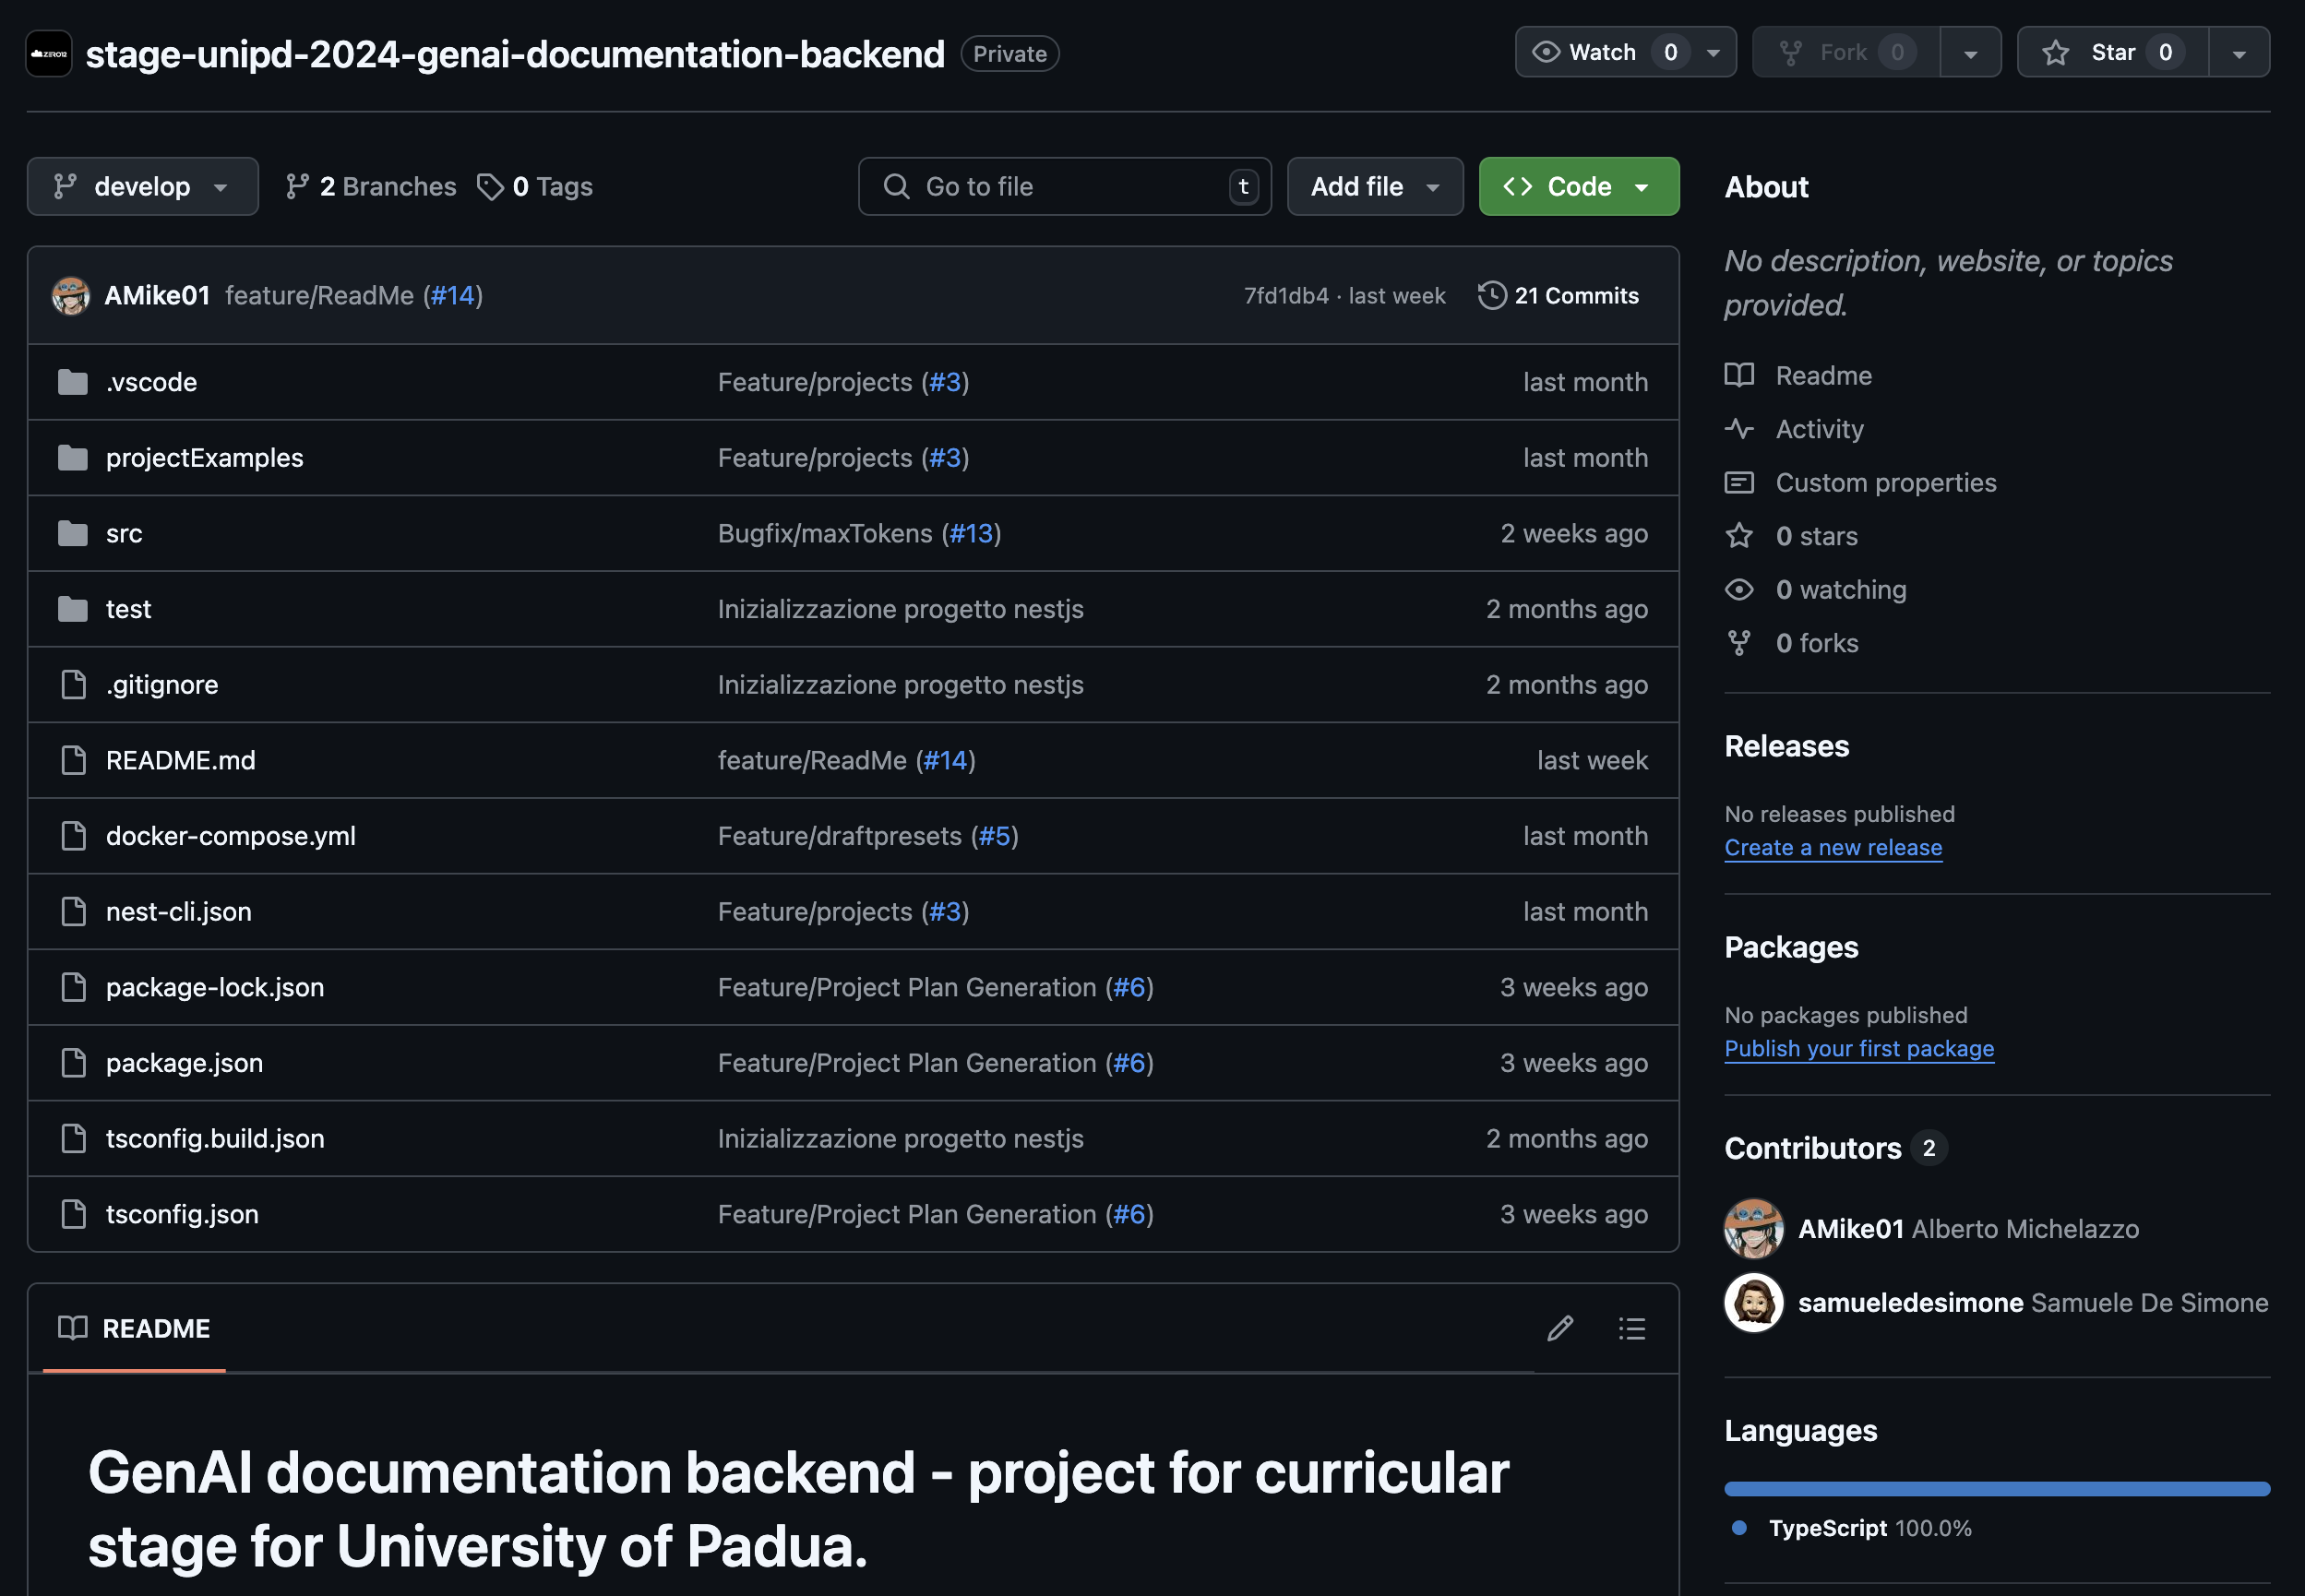
\includegraphics[scale=0.3]{strumenti/github-repo.png}
    \caption{\textit{GitHub} - Una delle \textit{repositories} create}
\end{figure}

\pagebreak

\subsubsection{Strumenti di comunicazione}
\label{sez:strumenti-comunicazione}

\noindent \textbf{Slack\\}

\noindent \textit{Slack} è un'applicazione di messaggistica istantanea che permette di comunicare con i propri colleghi in ambito aziendale. \\
Tramite la creazione di specifici canali è possibile organizzare le conversazioni per progetto, permettendo una comunicazione più efficace tra i membri del \textit{team}.\\
Come si può vedere nella {\hyperref[fig:slack]{Figura 1.4}}, nel caso del mio \textit{stage} è stato creato un canale dedicato al mio progetto, insieme al mio tutor ed ad un'altra figura aziendale, 
per poter comunicare in modo diretto e veloce in caso di problematiche o dubbi durante lo sviluppo.

\begin{figure}[H]
    \label{fig:slack} 
    \centering
    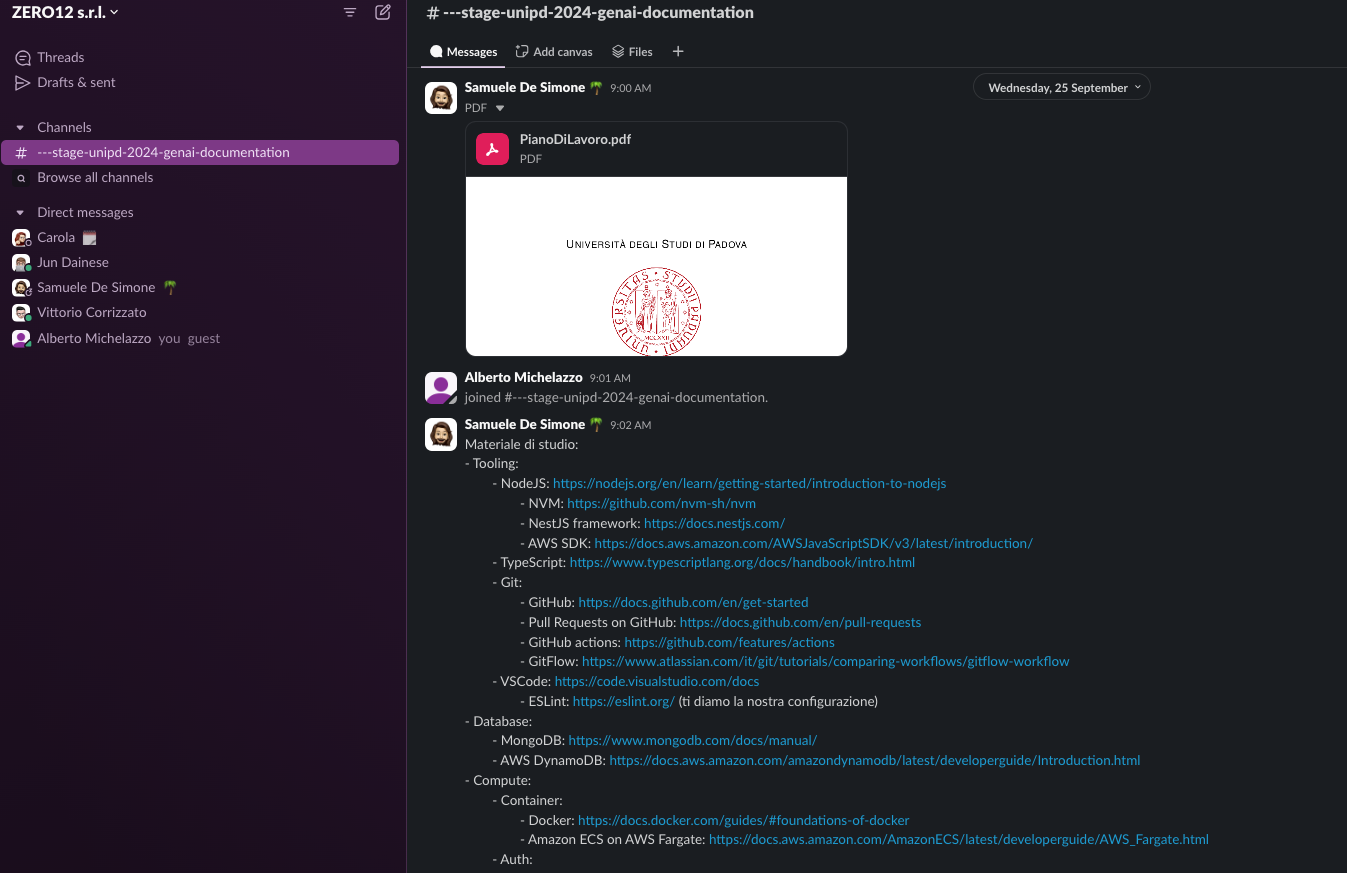
\includegraphics[scale=0.25]{strumenti/slack.png}
    \caption{\textit{Slack} - Canale dedicato al progetto}
\end{figure}

\noindent \textbf{Microsoft Teams\\}

\noindent \textit{Microsoft Teams} è un'applicazione di collaborazione che permette la comunicazione tra i membri del \textit{team}, la condivisione di \textit{file} e la gestione di riunioni.\\
Durante il mio \textit{stage} l'ho utilizzato per la gestione delle riunioni settimanali con il tutor aziendale, per discutere dello stato di avanzamento del progetto e per ricevere \textit{feedback} sul lavoro svolto, quando
non era possibile effettuare un incontro di persona.
